\documentclass[../full_thesis/full_thesis.tex]{subfiles}

% Default image directory
\newcommand{\thisdir}{../introduction}
\graphicspath{{\thisdir/img/}} 

\begin{document} 

Neutron stars were first postulated by Landau as `dense stars
which look like giant atomic nuclei' \citep{Yakovlev2013}, even before the
discovery of the neutron by \citet{Chadwick1932}. However it was
\citet{Baade1934} who made the explicit prediction of a neutron star whilst
trying to explain the energy released in observed supernova.

In a main-sequence star, the nuclear fusion of
hydrogen atoms into helium provides outward pressure balancing the star in an
equilibrium configuration with the inward pressure of the star's self-gravity.
Eventually the star depletes its reserves of hydrogen and can no longer
maintain equilibrium. If the star has an initial mass greater than $\sim 8
\Msun$, then it may undergo a \emph{core-collapse supernova} during which some
of the mass is ejected, but the rest falls in creating a new compact object.
In this object, temperatures and pressure rapidly soar and the
electrons and protons undergo inverse beta decay combining to form neutrons and
neutrinos:
\begin{equation}
    e^{-} + p \rightarrow n + \nu.
\end{equation}
If the compact object's mass is less than $M^{\textrm{max}}$, the maximum
mass of a stable neutron star found by \citet{oppenheimer1939massive},
then, once the pressure
reaches nuclear densities of $\sim 2.3 \times10^{14}$~g/cm$^{3}$, neutron
degeneracy pressure can halt the collapse in a new compact stable equilibrium
configuration which we call a neutron star. The exact value of $M^{\textrm{max}}$
depends on the equation of state of matter at high densities, but typical values
range from $1.5$, to $3 \Msun$ \citep{bombaci1996}.
For remnants with larger masses,
this is not possible and the object will collapse to form a black-hole; the
detail of exactly what the critical mass a neutron star can sustain is
sensitive to the equation of state of matter under these conditions.

Our knowledge of neutron stars is founded on observations made by
electromagnetic astronomy. This has revealed a wealth of different neutron
stars and their phenomena which we will introduce in the following sections.
Many of these observed phenomena have well defined models which allow us to
infer properties of neutron stars themselves.
However, our knowledge of neutron stars is far from complete: current
observations can be contradictory or have features not explained by any known
physical models. Improvements in electromagnetic astronomy will bring to light
a greater number of new neutron stars and improve the resolution of those
currently observed; it is hoped that this will help us to better understand them.

There are two other methods we can utilise to learn more about neutron stars: improved
modelling of current observations and by observing them from their
gravitational wave emissions. In this thesis, we will study how one of the
observed phenomena, so-called `timing variations', can help us to learn more
from current observations and also test whether it may hinder the current
search for gravitational waves from neutron stars.

In this introduction, we will acquaint the reader with the current observations
of neutron star and introduce some of the basic physics.

\section{Observation of pulsars and their identification with neutron stars}
After the conception of neutron stars as stable compact objects there was
thought to be little chance of observing them. They are many orders of
magnitude smaller than other celestial objects and soon after their formation
in rare supernovae events (the last observed event took place in 1604 and was
observed by Johannes Kepler) they are rapidly cooled by the emitted neutrinos
making their thermal emission difficult to detect.

In 1968 a bright periodic EM signal, now known as PSR~B1919+21, was identified
by \citet{Hewish1968} during a high time-resolution survey for interplanetary
scintillation. The source was measured with a radio radio frequency of 81.5~MHz
and pulsed with a period of $\sim 1.377$~s; this led to the name \emph{pulsars}
to refer to such sources.  Following this, several other similar objects where
discovered. A unifying feature of all pulsars is the clock-like stability of
the pulsations - something not rivalled by any other astrophysical phenomenon.
This stability indicates that the source must be a coliminated beam fixed to a
rotating body such that, as it rotates, the beam sweeps out like a lighthouse;
in this way the pulsation period is exactly the rotation period of the body.
Alternative models such as emission due to accretion from a binary companion
could never reach the stability's seen in pulsars.

For any rotating body to remain gravitationally bound, its rotation frequency is
constrained by the requirement that the centrifugal acceleration at the equator
be less than the gravitational acceleration. The rotation frequency of the observed
pulsars ruled out all known astrophysical bodies except the two most compact
objects, neutron stars and black holes, since all other bodies would not be
gravitationally bound at these frequencies. Isolated black holes are unable to
support an electromagnetic emission mechanism, this left only neutron stars
as candidates.

The identification of pulsars with neutron stars came independently from
\citet{Pacini1967} and \citet{Gold1968}. They suggested that a rapidly rotating
neutron star with a strong dipolar magnetic field would stream radiation out
along the magnetic axis. If this axis is misaligned from the rotation axis,
then the beams are swept out like a lighthouse. Beams passing over the earth
are observed as periodic pulses at the rotation frequency of the star.  Such a
model predicts that the electromagnetic radiation should exert a torque and
slow-down the rotation.  This slowdown was subsequently measured in the Crab
pulsar, which was discovered at the centre of the Crab nebulae which is a
supernova remnant, agreeing with the prediction of \citet{Baade1934}.

These early detection gave birth to a new field of astronomy: pulsar astronomy.
Since then, the field has detected over 2000 radio pulsars, measured thermal
emission from a handful of nearby neutron stars with typical temperatures of
$10^{5}$K to $10^{6}$K \citep{pavlov2003thermal}, found neutron stars in
accreting binary systems with companions, and identified many other ways to
observe neutron stars. We will discuss some of these which are relevant to this
thesis in Sec.~\ref{sec: categorising neutron stars}, but first in
Sec.~\ref{sec: pulsar timing methods} we describe the techniques used by the
field to identify and `time' radio pulsars.


\section{Pulsar timing}
\label{sec: pulsar timing methods}
Pulsars can be observed by measuring the variation in amplitude of the radio
waves from a particular sky location. A single observation consists of
measuring the amplitude over a time period of approximately $30$ minutes or so,
which, for pulsars with spin period~$\sim1$~s, means recording up to several
thousand individual pulsations.

The shape of individual pulses can vary substantially during a single
observation; to demonstrate this, in Figure~\ref{fig: CP1919 stacked},
successive pulses from PSR~B1919+21, the first discovered pulsar, are
vertically stacked and aligned.
\begin{figure}[htb]
\centering
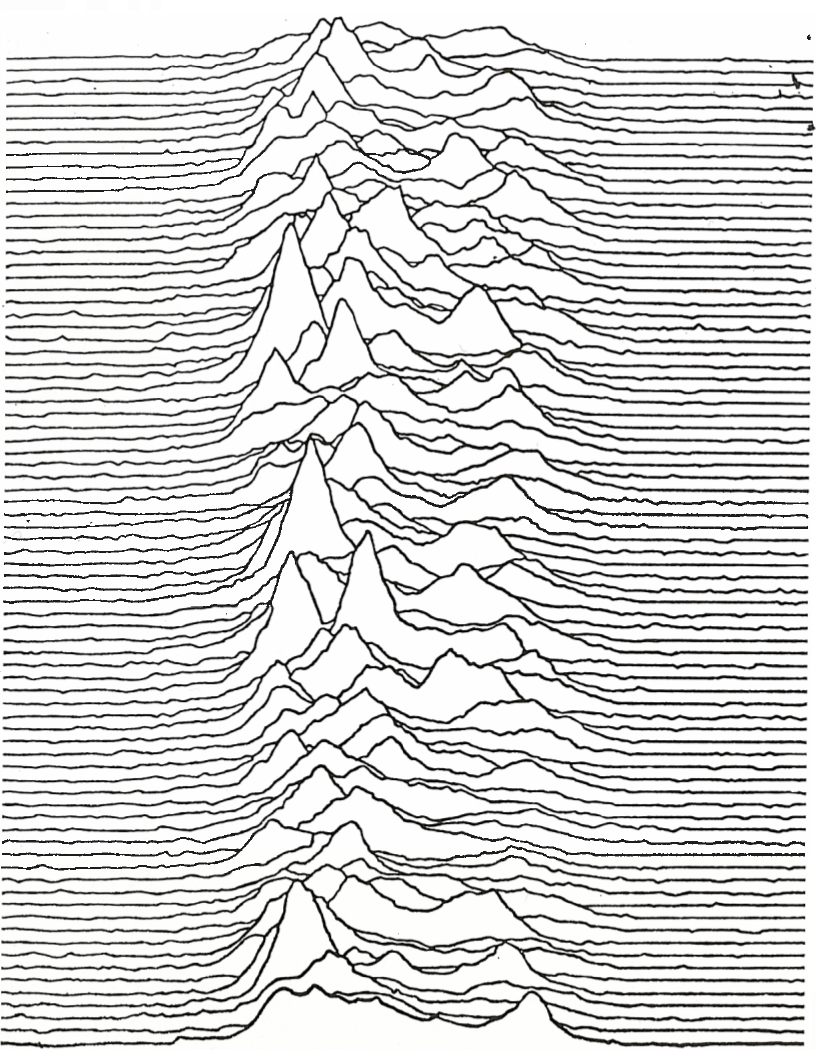
\includegraphics[width=0.5\textwidth]{CP1919_stacked}
\caption{The radio amplitude of successive pulses from PSR~B1919+21 stacked
vertically, figure reproduced from \citet{mitton1977cambridge}, originally
produced by \citet{craft1970}.}
\label{fig: CP1919 stacked}
\end{figure}
Each pulsation lasts for a small fraction of the pulse period. As an example,
the pulses in PSR~B1919+21, shown in Figure~\ref{fig: CP1919 stacked}, have
typical widths of $0.031$~s, but the pulse period is $1.337$~s; note that the
stacked plot is truncated to show only the pulsation itself. Later, in
Figure~\ref{fig: pop stats others}, we will show this to be a common
characteristic for the normal radio pulsar population by looking at the
duty-cycle, the ratio of the pulse duration to the pulse period.

In order to understand the gross features of a pulsar, astronomers average over
the hundreds to thousands of pulses observed during a single observation to
create a single integrated pulse profile. This is done by sampling the radio
signal at fixed time intervals then `folding' all the samples at the pulse
period (for a complete review see \citet{Lyne2012book}). In contrast to the
individual pulses which, as shown in Figure~\ref{fig: CP1919 stacked}, can be
highly variable, the integrated pulse profile is highly stable between
independent observations over timescales of years.

The integrated pulse profile not only gives a stable picture of what the
pulsations look like on average, but it also provides a highly accurate
measurement of the time of arrival (TOA) of a single pulse during the
observation. It is this TOA
which can be used to `time' a pulsar. To do this, regular observations of a
pulsar must be made every few months or so, with each observation resulting in a
precise TOA measurement. Having obtained a series of TOAs, pulsar astronomers
generate a \emph{timing model} which attempts to exactly count each and every
pulse. Between any two observations there may be several million pulses so the
timing model needs to account for any mechanisms which may produce variations
in the TOAs.  The process is standardised by the software package
\texttt{TEMPO2} developed by \citet{Hobbs2006}, of which we will now describe the
essential features.

The TOA of a pulse at the detector on Earth depends on many factors, such as: the
time at which the beam was directed by the source towards the Earth; the relative
motions of the source and detector; and any mechanisms effecting the signal during
its transit. In this thesis, we will be concerned only with the time at which
pulses are generated (when the source beams towards
the earth) which is governed by the \emph{timing properties} of the star itself.
As described by \citet{Edwards2006} these can be modelled by a Taylor expansion
in the phase at time $t$, given by
\begin{equation}
\phi(t) = \phi_0 + 2\pi \sum_{n\ge 1}\frac{\nu^{(n-1)}}{n!}(t - \tref)^{n},
\label{eqn: Taylor compact}
\end{equation}
where $\{\nu^{(n)}\}$ is the $n^\mathrm{th}$ time derivative of the spin
frequency of the rotating body, $\phi_0$ is the initial phase, and
$\tref$ is an arbitrary reference time. This expansion is usually truncated at
$n=3$, the second order spin-down rate $\ddot{\nu}$. The timing model then
includes corrections to this to model the relative motion of the source and
detector, intergalactic transit, and other effects; these are described in full
in \citet{Edwards2006}.

Between any two TOAs, if the timing model is correct, an integer number of
rotations must have occurred; this allows the use of the deviation of
$\phi(t_{TOA}^{j})$ from an integer as a test statistic. The timing model
minimises the root-mean-square (RMS) of these deviations with respect to the timing model
parameters, for example the frequency and frequency derivatives. The output of
applying a particular timing model (choice of corrections) to a set of data is
then the best-fit of these parameters and an estimate of their associated
errors.  The corrections applied in a timing model provide a method to
investigate pulsar physics: for example in some pulsars an orbital correction
must be applied which models the periodic motion of the star due to an orbital
companion. Using this technique, \citet{wolszczan1992planetary} discovered the
first \emph{exoplanets} orbiting the pulsar PSR~B1257+12.

A minimisation of the timing model parameters will converge regardless of
whether of not the model itself is appropriate. To qualitatively check if the
fitted model described the data, pulsar astronomers refer to the \emph{timing
residual}, which is the difference between the TOA, as given by the timing
model, and the actual TOA. The timing residual provides a mechanism to evaluate
the timing model: for example a periodic variation in the timing residual with period
$365$~days may indicate the correction of the Earth's orbit about the Sun may
be incorrect. If the timing model is correct, the residual data points should
be Gaussianly distributed around zero. A timing model is described as
\emph{phase-connected} if it is accurate enough to track the pulsar to within a
single rotation. For most pulsars this is the case and a single set of
coefficients can track the spin-down over periods greater than a year.

However, for all pulsars the timing residual contains `structure' known as
\emph{timing variations} which cannot be associated with any known correction.
These variations are the focus of this work and we will describe the details
further in Section~\ref{sec: timing variations}.  In the next section, we will
describe the variety of known pulsars which have been timed using this method.




\section{Categorising neutron stars}
\label{sec: categorising neutron stars}
The timing properties, and other features measured by the timing model, for
over 2000 pulsars observed can be accessed via the ATNF pulsar catalogue
\citep{ATNF}.  We can categorise the population by their measured values of
period $P$ and period derivative $\Pdot$. This is done by plotting them in a
so-called $P - \Pdot$ diagram as shown in Fig.~\ref{fig: Period_PeriodDot}.
Some of the pulsar varieties have been marked in this plot and we now discuss
their features.

\begin{figure}[hb]
    \centering
    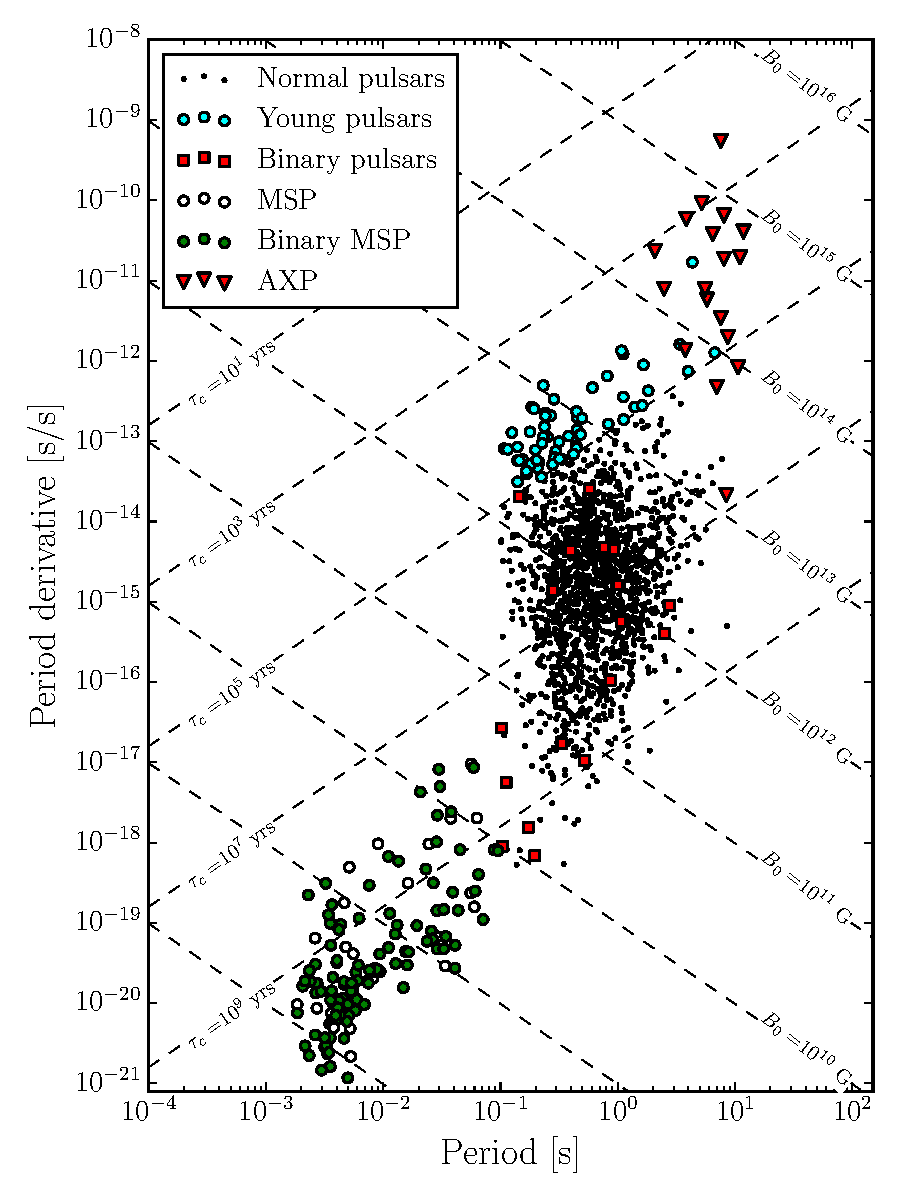
\includegraphics[width=0.8\textwidth]{Period_PeriodDot}
    \caption{Period - period diagram using data taken from the ATNF pulsar
             catalogue \citep{ATNF}. Dashed lines show inferred magnetic fields
             and characteristic ages as described in Sec.~\ref{sec: rotation
             powered pulsars}}
    \label{fig: Period_PeriodDot}
\end{figure}

The majority of pulsars, referred to as the `normal' pulsars, are
\emph{isolated} (without a binary companion) and have typical periods of
$P=10^{-1}-10^{1}$~s. These can be described as \emph{rotation powered} pulsars
since the EM radiation is powered by the loss of rotational energy. As
described later in Sec.~\ref{sec: rotation powered pulsars}, estimates can be made
for their characteristic age $\tau_{c}$ and surface magnetic field strength
$B_{0}$ based on a dipole spin-down model. Constant lines of these quantities
are plotted in Fig.~\ref{fig: Period_PeriodDot}. Of the normal pulsars, we
can identify the young pulsars as those for which $\tau_{c}<10^{5}$~yrs. Some
of these, such as the Crab and Vela, can be directly associated with their
supernova remnant from which they were formed \citep{Kaspi1996}.

A second smaller population of isolated rotation powered pulsars exists with
$P<10^{-1}$~s, these are the \emph{millisecond pulsars} (MSPs). These special
class of pulsars are believed to start life as normal pulsars, but are then
spun-up through accretion from a normal star. In support of this hypothesis,
the majority of MSPs in figure \ref{fig: Period_PeriodDot} have a binary
companion \citep{wijnands1998millisecond}.  During the accretion stage, the
mechanism responsible for the electromagnetic emission is thought to switch-off
and so we do not see their pulsations. However, we can observe them in an X-ray
binary when they undergo outburst \citep{lewin1997x}; this is caused by the
heating of material in the accretion disk as the neutron star draws material
from the companion star.

Some isolated pulsars are observed as sporadic bursts of pulsed X-ray radiation,
these are known as anomalous X-ray pulsars (AXPs). The neutron stars which are
thought to produce this emission have large magnetic fields $B_{0}\gtrsim
5\times10^{13}$; as a result they are named \emph{magnetars}. The high energy
radiation is thought to result from the decay of this magnetic field.


\section{Radio pulsar population statistics}
\label{sec: population stats}
Radio pulsars make up the majority of observations of neutron stars and will be
the focus of discussion in this thesis. In this section, we will provide some
population statistics for the normal radio pulsar population: we ignore the
millisecond population, but include the young pulsars. All data
in this section is taken from the ATNF pulsar catalogue \citet{ATNF} and it
should be stated that in each case the observed property is an average
over all observations made for each pulsar.

For each observable property of the population of neutron stars (such as the
frequency), we will present the data as a histogram choosing an appropriate
binning size in each instance. In order to make simple inferences about the
population, we also give the mean and standard-deviation and plot the
corresponding normal distribution.

In Fig.~\ref{fig: pop stats timing} we present the data for the three timing
properties measured directly from the pulsar timing models. For normal radio
pulsars the frequency, $f$, can always be accurately measured provided at least
one observation has been made.  Several precise observations of a pulsar must
be made in order to measure the higher order derivatives of the frequency. As a
result, the pulsar catalogue contains missing information and the number of
data points for $\dot{f}$ and $\ddot{f}$ is smaller than the total observed
number of pulsars: the exact numbers are given in the caption.
\begin{figure}[htb]
\centering
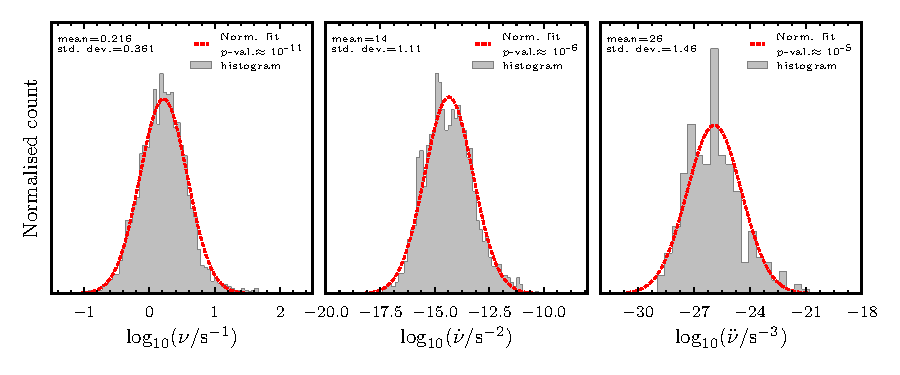
\includegraphics[]{timing_distribution}
\caption{The distribution in log-space of the frequency $f$ and the first two
frequency derivatives $\dot{f}$ and $\ddot{f}$ for normal radio pulsars in the
ATNF pulsar catalogue. Appropriate bin sizes were selected for each quantity.
The population sizes are 1942, 1686, 339 for $f$,
$\dot{f}$, $\ddot{f}$ respectively.}
\label{fig: pop stats timing}
\end{figure}

In Fig.~\ref{fig: pop stats others} we present some other interesting quantities
held in the ATNF catalogue. Firstly, in the left-hand panel we plot the characteristic
age as defined in Eqn.~\eqref{eqn: characteristic age}. Then, in the middle panel
we give a measure of the pulsars beam-width $W_{10}$. Specifically, $W_{10}$ is
the width of the integrated pulse profile (in seconds) at 10\% of the integrated
pulse profile maximum. In the right-hand panel we  plot $W_{10}f$, i.e. the
product of the beam-width and frequency for each pulsar. This gives information
about the effective duty-cycle: the ratio between the pulse duration and period.
Notably, the majority of pulsars have duty-cycles substantially less than a
$0.5$ indicating that the pulses are short compared to the period.
\begin{figure}[htb]
\centering
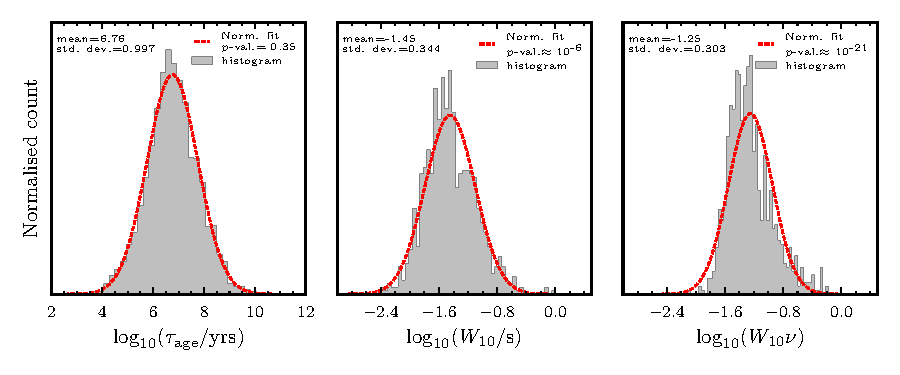
\includegraphics[]{W10_and_age_distribution}
\caption{The distribution in log-space of the characteristic age
$\tau_{\textrm{Age}}$, the $W_{10}$ measure of the beam-width, and the
effective duty-cycle $W_{10} f$ for normal radio pulsars in the
ATNF pulsar catalogue. Appropriate bin sizes were selected for each quantity.
The population sizes are 1942, 915, and 915 for
$\tau_{\textrm{Age}}$, $W_{10}$, and $W_{10}f$.}
\label{fig: pop stats others}
\end{figure}



\section{The physics of rotation powered pulsars} 
\label{sec: rotation powered pulsars}
For rotation powered pulsars, the normal population in Fig.~\ref{fig:
Period_PeriodDot}, we describe in this section how the neutron star properties
can be inferred from the stars timing properties. To do this, we will model the
star as described by \citet{Pacini1967} and \citet{Gold1968} and illustrated in
Fig.~\ref{fig: DipoleSpindownSimple}: a rapidly rotating
body with a magnetic dipole fixed in the crust at an angle $\alpha$ to the rotation
axis.
\begin{figure}[htb]
    \centering
    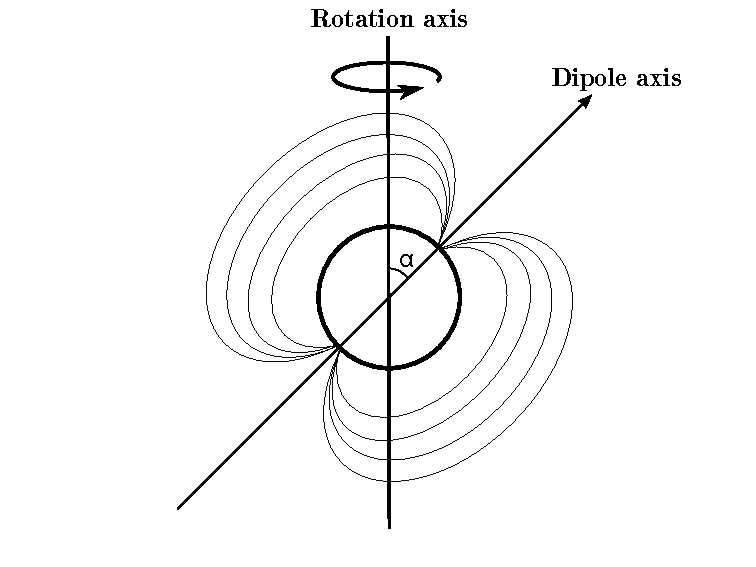
\includegraphics[width=.5\textwidth]{DipoleModelSimple}
    \caption{An illustration of the dipole spin-down model. The dipole and some 
    of the closed field lines are fixed at an angle $\alpha$ to the rotation 
    axis. As the body rotates, radiation is emitted along both ends of the dipole
    axis producing a torque on the body.}
    \label{fig: DipoleSpindownSimple}
\end{figure}

From \citet{Landau2013classical} the total radiation from a dipole rotated at
angular frequency $\Omega$ is given by
\begin{align}
I = \frac{2}{3}\frac{\Omega^{4}}{c^{3}} d_{0}^{2},
\end{align}
where $d_0$ is the projection of the dipole moment on the plane perpendicular
to the axis of rotation \citep{Pacini1967}. Following \citet{Shapiro83}, the
magnitude of the magnetic dipole moment for a star with radius $R$ and surface magnetic
field strength $B_0$ is $B_{0}R^{3}/2$. Including the projection onto the
plane perpendicular to the rotation axis, the total radiation is then
\begin{align}
I = \frac{1}{6}\frac{\Omega^{4}}{c^{3}} B_0^2 R^{6} \sin^{2}\alpha.
\end{align}

The rotational energy of a body spinning at $\Omega$ with a moment of inertia
$I_{0}$ is given by
\begin{equation}
    E = \frac{1}{2}I_{0}\Omega^{2}.
\end{equation}
Differentiating this expression with respect to time gives the loss of rotational
energy, $\dot{E}=I_0 \Omega\dot{\Omega}$. Assuming that all the energy is lost
to the rotation of the dipole, hence the name rotation powered pulsars, we can
equate $\dot{E} = -I$. We then rearrange
to give a power-law relation between the spin-down rate and the spin-frequency:
\begin{align}
\dot{\Omega} = -\frac{B_0^{2} R^{6} \sin^{2}\alpha}{6 c^{3} I_0} \Omega^{3}.
\end{align}

This power-law dependence is a model specific version of a more general
phenomenological power-law braking model
\begin{equation}
    \dot{\Omega} = -k \Omega^{n}.
    \label{eqn: power law spin-down}
\end{equation}
Generalising in this way suggests a powerful method to determine the type of
braking for a given pulsar. Specifically, differentiating Eqn.~\eqref{eqn: power law spin-down}
and rearranging it can be shown that
\begin{equation}
    n = \frac{\ddot{\Omega}\Omega}{\dot{\Omega}^{2}}.
    \label{eqn: measured braking index}
\end{equation}
Therefore, if $\ddot{\Omega}$ can be measured, then $n$ can be determined, and
hence used to infer the type of braking. For example, measuring $n=3$ would
indicate the pulsar braking is dominated by losses due to the magnetic dipole,
in contrast, it can be shown that gravitational wave braking would produce
$n=5$ \citep{Shapiro83}. Unfortunately, in reality, pulsars do not constrain this
value. Braking indexes have been measured with values as large as $\sim10^{6}$.
We will return to this issue in Sec.~ \ref{sec: evidence from anomalous braking
indices}.

To infer the age of the pulsar, Eqn.~\eqref{eqn: power law spin-down} can
be integrated between the initial values ($t=0, \Omega=\Omega_{i}$) and the
observed value ($\Omega_{\mathrm{o}}$) to give
\begin{equation}
    t = \frac{1}{(1-n)} \frac{\Omega_{\mathrm{o}}}{\dot\Omega_{\mathrm{o}}} 
        \left(1 - \frac{\Omega_{\mathrm{o}}^{n-1}}{\Omega_{i}^{n-1}}\right).
\label{eqn: characteristic age}
\end{equation}
Typically, we make the assumption that all
pulsars, regardless of their measure braking index, are dominated by EM braking
such that $N=3$. Then additionally assuming that $\Omega_{i} \gg
\Omega_{\mathrm{o}}$ we can approximate to a characteristic age
\begin{equation}
    \tau_c = \frac{-1}{2}\frac{\Omega_{\mathrm{o}}}{\dot\Omega_{\mathrm{o}}}
         = \frac{1}{2}\frac{P}{\Pdot},
\end{equation}
where $P=\frac{2\pi}{\Omega}$ is the pulse period and
$\dot{P}=-2\pi\frac{\dot{\Omega}}{\Omega^{2}}$ is the period derivative.

To infer the approximate surface magnetic field strength, we first note that
in the EM dipole braking model:
\begin{align}
k = \frac{B_0^{2} R^{6} \sin^{2}\alpha}{6c^{3}I_0}.
\end{align}
Then rearranging and substituting for $k$ in Eqn.~\eqref{eqn: power law
spin-down} we can estimate the surface magnetic field strength by
\begin{equation}
    B_{0} = \left(\frac{6 c^{3} I_{0}}{R^{6} \sin^{2}\alpha}\right)^{\frac{1}{2}} 
            \left(\frac{-\dot{\Omega}}{\Omega^{3}}\right)^{\frac{1}{2}}
          = \frac{1}{2\pi}\left(\frac{6 c^{3} I_{0}}{R^{6} \sin^{2}\alpha}\right)^{\frac{1}{2}}
           \sqrt{P \Pdot}
\label{eqn: surface magnetic field}
\end{equation}
In general we do not know the inclination angle $\alpha$, but we can evaluate a 
minimum magnetic field strength by setting $\alpha=\pi/2$. In CGS units, for a
canonical pulsar with $R=10^{6}$~cm, $I_{0}=10^{45}$~g~cm$^{2}$ \citep{Lyne2012book}, we can approximate
the magnetic field strength as
\begin{equation}
    B_{0} = 3.2 \times 10^{19} \sqrt{P \Pdot}.
\label{eqn: surface magnetic field canonical}
\end{equation}

In this section, we have introduced some of the simple results that can be
obtained by modelling the time evolution of pulsars with a power law. In
practise this model is consisent with most pulsar observations and provides a
useful way to categorise them via their spin-down age and magnetic field.
However, such a model does not capture all of the subtle variations which are
the focus of this thesis.  We will frequently refer back to this model as it
provides a useful platform from which to begin understanding neutron stars.



\section{Neutron stars and gravitational waves}
\label{sec: gravitational waves}
Gravitational waves (GWs) were first predicted by Albert Einstein in 1916
\citep{einstein1916approximative} when he found that the linearised weak-field
equations of his General Theory of Relativity had transverse wave solutions.
Much like the generation of electromagnetic waves requires the acceleration of
electrical charges, GWs are generated by any source with a
time-varying mass quadrupole moment and can be understood as `ripples' or
spatial strains in the spacetime itself which travel at the speed of light.

Gravitational waves were first directly detected by the LIGO collaboration
\citep{abbott2016observation}. They observed a signal consistent with the
inspiral and merger event of two $\sim 30 \Msun$ black-holes over approximately
$0.2$~s. To detect such signals, LIGO uses a \emph{laser interferometer} to
measures the relative change in length between two orthogonal arms. In
particular, if $L$ is the length of either arm without a signal and a
gravitational wave passes through, the detector measures the strain
\begin{align}
h(t) = \frac{\delta L_x - \delta L_y}{L}
\end{align}
where $\delta L_x$ and $\delta L_y$ are the time-varying stretching and
squeezing of the two arms caused by the gravity wave. For the observed binary
black-hole merger the peak strain in the detector was $\sim 10^{-21}$.

Prior to this detection, indirect evidence for the existence of gravitational
waves was found by observing the orbital periods of compact binary systems.
Such systems have a time-varying quadrupole moment and emit gravitational
waves, which radiate energy away from the system causing, a decay of the orbital
period. In 1975, Hulse \& Taylor discovered a binary neutron star system where
one of the stars, PSR~B1913+16, was visible as a pulsar \citep{Hulse1975}. Due to
the powerful techniques of pulsar timing, subsequent analysis by
\citet{Taylor1982} was able to verify that the orbital decay matched exactly
the predictions of General Relativity. Since this observation, more double
neutron star system have been discovered, including a system, PSR~J0737-3039A/B,
discovered by \citet{burgay2003increased}, where both neutron stars are seen as
pulsars. This so-called double pulsar system tests the agreement with General
Relativity at the 0.05\% level \citep{kramerstairs2006}.

Neutron stars observed as pulsars are often referred to as `cosmic clocks' for
the regularity of their pulsations. The most stable pulsars are the radio
millisecond pulsars (MSPs), which, due to their stability, many workers in the field
utilise in an attempt to search for GWs via a \emph{pulsar timing array}
\citep{hobbs2010international}: this searches for correlated signatures in the
TOAs from a network of well-timed MSPs. Such a detector is sensitive to a
stochastic background of gravitational waves by measuring the so-called
Hellings \& Downs curve \citep{hellings1983upper}, or to the mergers of
super-massive black hole binary systems \citep{lee2011gravitational}.

Isolated neutron stars themselves are potential sources of gravitational waves
through one of three mechanisms. If the star has a rotation axis misaligned
with its symmetry axis then it will undergo \emph{precession}: a `wobble` of
the star which has a time-varying quadrupole moment. This will produce GWs at
the rotation frequency and twice the rotation frequency, but the small
amplitudes of possible sources and questions over how long lived they might be
make this an unlikely candidate for LIGO \citep{Jones2002}. If the neutron star
is subject to \emph{non-axisymmetric instabilities}, such as the r-mode
instability in newborn and rapidly accreting neutron stars
\citep{andersson2001r}, then these too can produce GWs (for a review see
\citet{andersson2003gravitational}).  Finally, if the star possesses a
\emph{non-axisymmetric distortion}, $\epsilon$, also known as a `mountain', it
will produce a continuous gravitational wave at twice its rotation frequency
with a strain amplitude proportional to $\epsilon$. The LIGO detectors have
already been used to search for signals from known neutron stars and, by not
observing any radiation, are able to place upper limits on $\epsilon$ (see for
example \citet{abbott2008beating, abadie2011beating}).

All three of these detection mechanisms are potential sources of the first
detection of gravitational waves from neutron stars and realising this would
provide a unique opportunity to learn about neutron stars. But is it feasible?
A statistical argument can be made for the `loudest expected signal from
unknown isolated neutron stars'. This argument is given in
\citet{abbott2007searches}, although the origin can be dated back to Blandford
(1984) as attributed by Kip Thorne in \citet{Hawking1989}. Essentially, one
makes the assumption that the population of $10^{5}$ neutron stars predicted to
exist in our galaxy by stellar evolution models are all born with a high
spin-down rate and subsequently spin-down principally due to the emission of
gravitational waves. With additional assumptions that the stars are born
randomly throughout the Galactic disk with a constant birthrate the populations
are transformed into a population of neutron star strains. Then it is shown
that there is a 50\% chance a source exists with a strain amplitude
\begin{align}
h_0 \sim 4 \times 10^{-24},
\end{align}
which is close to `detectable' by LIGO, although the exact details depend on the
source frequency and duration. While this is a purely statistical argument, and
changing any of the assumptions tends to decrease this signal strain
\citep{Prix2009}, the rewards for detection in terms of astrophysics are
sufficient to motivate further research.




\section{Plan of the thesis}

Following this introductory chapter, we will introduce so-called timing
variations in pulsars: glitches and timing-noise. This will familiarise the
reader with observed phenomena and describe the current state of modelling.  We
will provide some original work on simple ways in which the models could be
tested.

In the next four chapters we evaluate models of timing noise in the face of
current observations and attempt to constrain the models.  In Chapter~\ref{sec:
rotating frame} we explore how \emph{precession}, a potential ingredient to
explain timing-noise, can be described, when viewed from the frame rotating
with the star. Following this, Chapter~\ref{sec: rotating frame} looks at how
precession will manifest in the observations made by pulsar astronomers. In
Chapter~\ref{sec: testing models} we perform a rigorous quantitative model
comparison between precession and the leading alternative, \emph{switching},
for describing timing variations seen in PSR~B1828-11.

In the final three chapters we approach another important aspect of timing
variations for neutron stars: the effect they may have on our ability to detect
gravitational waves from neutron stars. In Chapter~\ref{sec: intro to cgw} we
introduce the methods and formalisms used by gravitational wave astronomy
before analysing the effect of glitches on gravitational wave searches in
Chapter~\ref{sec: glitches in cgw}. For the effect of timing-noise on
gravitational wave searches, we perform a numerical study on data from the Crab
pulsar in Chapter.~\ref{sec: timing noise in cgw} and then model the effect of
different timing noise interpretations in Chapter.~\ref{sec: timing noise in
cgw analytic}. Finally, we will conclude in Chapter.~\ref{sec: conclusion}.

\biblio


\end{document}
